\documentclass{standalone}
\usepackage{fontspec}
\setsansfont{DejaVuSans.ttf}[Path=./,Kerning=Off,Ligatures={TeXOff,NoCommon}]
\usepackage{tikz}
\begin{document}
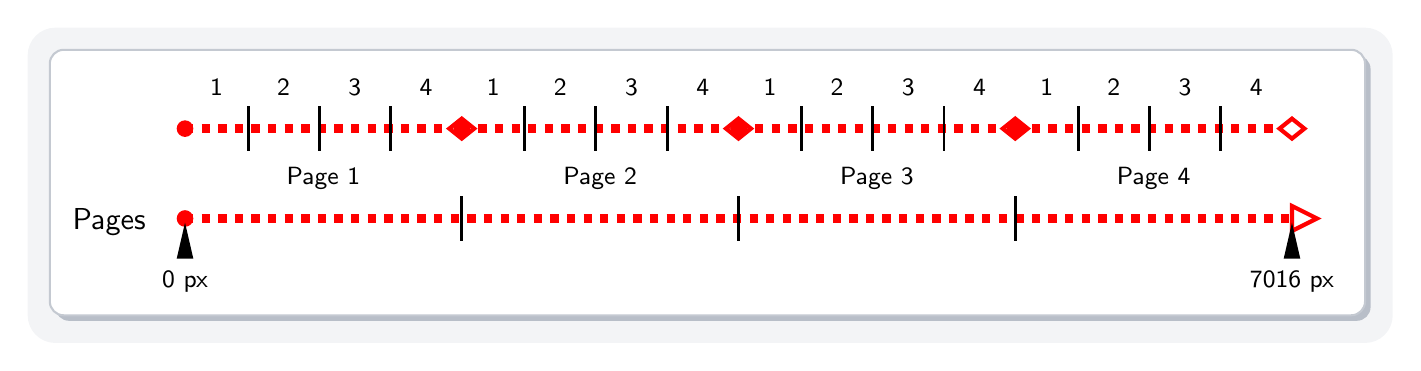
\begin{tikzpicture}[x=1pt,y=1pt,miter limit=4,font=\sffamily]
\definecolor{ts000000}{HTML}{000000}
\definecolor{tsB8BEC8}{HTML}{B8BEC8}
\definecolor{tsC4C9D1}{HTML}{C4C9D1}
\definecolor{tsF3F4F6}{HTML}{F3F4F6}
\definecolor{tsFF0000}{HTML}{FF0000}
\definecolor{tsFFFFFF}{HTML}{FFFFFF}
\begin{scope}[shift={(16,16)}]
\path[rounded corners=10pt,fill=tsF3F4F6] (0,0) rectangle (493.2571,113.9297);
\path[rounded corners=5pt,fill=tsB8BEC8] (10,8) rectangle (485.2571,103.9297);
\path[rounded corners=5pt,fill=tsFFFFFF,draw=tsC4C9D1,line width=0.75pt] (8,10) rectangle (483.2571,105.9297);
\path[draw=tsFF0000,line width=3pt,dash pattern=on 3pt off 3pt] (56.855,44.9766) -- (456.855,44.9766);
\path[fill=tsFF0000] (56.855,44.9766) circle[radius=3];
\path[draw=tsFF0000,line width=1.5pt] (465.855,44.9766) -- (456.855,49.4766) -- (456.855,40.4766) -- cycle;
\path[draw=tsFF0000,line width=3pt,dash pattern=on 3pt off 3pt] (56.855,77.4531) -- (152.355,77.4531);
\path[fill=tsFF0000] (56.855,77.4531) circle[radius=3];
\path[draw=tsFF0000,line width=1.5pt] (152.355,77.4531) -- (156.855,81.0531) -- (161.355,77.4531) -- (156.855,73.8531) -- cycle;
\path[draw=tsFF0000,line width=3pt,dash pattern=on 3pt off 3pt] (156.855,77.4531) -- (252.355,77.4531);
\path[fill=tsFF0000] (156.855,77.4531) circle[radius=3];
\path[draw=tsFF0000,line width=1.5pt] (252.355,77.4531) -- (256.855,81.0531) -- (261.355,77.4531) -- (256.855,73.8531) -- cycle;
\path[draw=tsFF0000,line width=3pt,dash pattern=on 3pt off 3pt] (256.855,77.4531) -- (352.355,77.4531);
\path[fill=tsFF0000] (256.855,77.4531) circle[radius=3];
\path[draw=tsFF0000,line width=1.5pt] (352.355,77.4531) -- (356.855,81.0531) -- (361.355,77.4531) -- (356.855,73.8531) -- cycle;
\path[draw=tsFF0000,line width=3pt,dash pattern=on 3pt off 3pt] (356.855,77.4531) -- (452.355,77.4531);
\path[fill=tsFF0000] (356.855,77.4531) circle[radius=3];
\path[draw=tsFF0000,line width=1.5pt] (452.355,77.4531) -- (456.855,81.0531) -- (461.355,77.4531) -- (456.855,73.8531) -- cycle;
\path[draw=ts000000,line width=1pt] (79.66,85.4531) -- (79.66,69.4531);
\path[draw=ts000000,line width=1pt] (105.3156,85.4531) -- (105.3156,69.4531);
\path[draw=ts000000,line width=1pt] (131.0853,85.4531) -- (131.0853,69.4531);
\path[draw=ts000000,line width=1pt] (156.855,52.9766) -- (156.855,36.9766);
\path[draw=ts000000,line width=1pt] (179.66,85.4531) -- (179.66,69.4531);
\path[draw=ts000000,line width=1pt] (205.3156,85.4531) -- (205.3156,69.4531);
\path[draw=ts000000,line width=1pt] (231.0853,85.4531) -- (231.0853,69.4531);
\path[draw=ts000000,line width=1pt] (256.855,52.9766) -- (256.855,36.9766);
\path[draw=ts000000,line width=1pt] (279.66,85.4531) -- (279.66,69.4531);
\path[draw=ts000000,line width=1pt] (305.3156,85.4531) -- (305.3156,69.4531);
\path[draw=ts000000,line width=1pt] (331.0853,85.4531) -- (331.0853,69.4531);
\path[draw=ts000000,line width=1pt] (356.855,52.9766) -- (356.855,36.9766);
\path[draw=ts000000,line width=1pt] (379.66,85.4531) -- (379.66,69.4531);
\path[draw=ts000000,line width=1pt] (405.3156,85.4531) -- (405.3156,69.4531);
\path[draw=ts000000,line width=1pt] (431.0853,85.4531) -- (431.0853,69.4531);
\path[fill=ts000000] (56.855,43.4766) -- (53.855,30.4766) -- (59.855,30.4766) -- cycle;
\path[fill=ts000000] (456.855,43.4766) -- (453.855,30.4766) -- (459.855,30.4766) -- cycle;
\node[anchor=base west,inner sep=0,font=\sffamily\fontsize{11}{12.8047}\selectfont,text=ts000000] at (16,41.1685) {Pages};
\node[anchor=base,inner sep=0,font=\sffamily\fontsize{9}{10.4766}\selectfont,text=ts000000] at (56.855,20.1226) {0 px};
\node[anchor=base,inner sep=0,font=\sffamily\fontsize{9}{10.4766}\selectfont,text=ts000000] at (456.855,20.1226) {7016 px};
\node[anchor=base,inner sep=0,font=\sffamily\fontsize{9}{10.4766}\selectfont,text=ts000000] at (106.855,57.0991) {Page 1};
\node[anchor=base,inner sep=0,font=\sffamily\fontsize{9}{10.4766}\selectfont,text=ts000000] at (68.2575,89.5757) {1};
\node[anchor=base,inner sep=0,font=\sffamily\fontsize{9}{10.4766}\selectfont,text=ts000000] at (92.4878,89.5757) {2};
\node[anchor=base,inner sep=0,font=\sffamily\fontsize{9}{10.4766}\selectfont,text=ts000000] at (118.2005,89.5757) {3};
\node[anchor=base,inner sep=0,font=\sffamily\fontsize{9}{10.4766}\selectfont,text=ts000000] at (143.9701,89.5757) {4};
\node[anchor=base,inner sep=0,font=\sffamily\fontsize{9}{10.4766}\selectfont,text=ts000000] at (206.855,57.0991) {Page 2};
\node[anchor=base,inner sep=0,font=\sffamily\fontsize{9}{10.4766}\selectfont,text=ts000000] at (168.2575,89.5757) {1};
\node[anchor=base,inner sep=0,font=\sffamily\fontsize{9}{10.4766}\selectfont,text=ts000000] at (192.4878,89.5757) {2};
\node[anchor=base,inner sep=0,font=\sffamily\fontsize{9}{10.4766}\selectfont,text=ts000000] at (218.2005,89.5757) {3};
\node[anchor=base,inner sep=0,font=\sffamily\fontsize{9}{10.4766}\selectfont,text=ts000000] at (243.9701,89.5757) {4};
\node[anchor=base,inner sep=0,font=\sffamily\fontsize{9}{10.4766}\selectfont,text=ts000000] at (306.855,57.0991) {Page 3};
\node[anchor=base,inner sep=0,font=\sffamily\fontsize{9}{10.4766}\selectfont,text=ts000000] at (268.2575,89.5757) {1};
\node[anchor=base,inner sep=0,font=\sffamily\fontsize{9}{10.4766}\selectfont,text=ts000000] at (292.4878,89.5757) {2};
\node[anchor=base,inner sep=0,font=\sffamily\fontsize{9}{10.4766}\selectfont,text=ts000000] at (318.2005,89.5757) {3};
\node[anchor=base,inner sep=0,font=\sffamily\fontsize{9}{10.4766}\selectfont,text=ts000000] at (343.9701,89.5757) {4};
\node[anchor=base,inner sep=0,font=\sffamily\fontsize{9}{10.4766}\selectfont,text=ts000000] at (406.855,57.0991) {Page 4};
\node[anchor=base,inner sep=0,font=\sffamily\fontsize{9}{10.4766}\selectfont,text=ts000000] at (368.2575,89.5757) {1};
\node[anchor=base,inner sep=0,font=\sffamily\fontsize{9}{10.4766}\selectfont,text=ts000000] at (392.4878,89.5757) {2};
\node[anchor=base,inner sep=0,font=\sffamily\fontsize{9}{10.4766}\selectfont,text=ts000000] at (418.2005,89.5757) {3};
\node[anchor=base,inner sep=0,font=\sffamily\fontsize{9}{10.4766}\selectfont,text=ts000000] at (443.9701,89.5757) {4};
\end{scope}
\end{tikzpicture}
\end{document}
